\section{Red-Black Tree}

\subsection{Definition and Properties}

\vspace{\parskip}

\begin{definition}[Red-Black Tree] \index{red-black tree}
    A red-black tree is a binary search tree in which every node is either red or black and satisfies the following properties:
    \begin{enumerate}
        \item The root is black
        \item Every leaf node (\textsc{nil} node) is black
        \item If a node is red, then both its children are black
        \item For each node, all paths from the node to descendant leaves (\textsc{nil} nodes) contain the same number of black nodes
    \end{enumerate}
    Alternatively, the properties can be stated without using the \textsc{nil} node.
    \begin{enumerate}
        \item The root is black
        \item A red node has no red children
        \item Every path from the root to a node with at most one child contains the same number of black nodes
    \end{enumerate}
\end{definition}

Figure \ref{fig:rbtree} illustrates the properties of red-black trees.

\begin{figure}[hp]
    \centering
    \includegraphics[width=\linewidth]{rbtree_nil.pdf}
    \includegraphics[width=\linewidth]{rbtree.pdf}
    \caption{Red-black trees. The first tree is represented with the \textsc{nil} sentinel node. The second tree is without the \textsc{nil} node. The two trees are equivalent and both satisfies the red-black tree properties.}
    \label{fig:rbtree}
\end{figure}

\begin{lemma}
    The number of nodes in a red-black tree of height $h$ is at least $2^{\left\lceil (h+1)/2 \right\rceil} - 1$.
\end{lemma}

\begin{proof}

    A red-black tree of height $h$ has a path of length $h$ from the root to a leaf node. This path contains $h+1$ nodes, the first of which is black. Since it does not contain two consecutive red nodes, the path contains at least $b = \left\lceil (h+1)/2 \right\rceil $ black nodes (i.e. at least half of the nodes on that path are black). Hence, every path from the root to a node with at most one child contains at least $b$ black nodes.
    It suffices to prove that there are at least $2^b-1$ black nodes in a red-black tree of height $h$ such that the number of black nodes in the path from the root to a leaf node is $b$. 

    \textsc{Base Case:} If the height of the tree is $0$, then the number of nodes is $1$.

    \textsc{Inductive Step:} Let $h \in \N$ be arbitrary. Assume that for all tree with height $h' < h$, there are $2^{b'}-1$ black nodes where $b'$ is the number of black nodes in the path from the root of that tree to a leaf node. 

    Consider an arbitrary tree $T$  with height $h$ with two subtrees. It follows that there are $b = \left\lceil (h+1)/2 \right\rceil$ black nodes from the root of the tree to a leaf node. If the subtree has a black root, then the path going from the root of the subtree to a leaf contains $b-1$ black nodes. If the root is red, then the path contains $b$ black nodes. Therefore, the number of black nodes in the path from the root of the tree to a leaf node is $b-1$ or $b$. Then, by induction hypothesis, the number black nodes in each subtree is at least $2^{b-1}-1$.

    Since the root of a red-black tree is black, the number of black nodes in $T$ is the number of nodes in the left subtree plus the number of nodes in the right subtree plus the root node.

    $$
    \left( 2^{b-1}-1 \right) + \left( 2^{b-1}-1 \right) + 1 = 2^{b}-1
    $$

    By induction, the number of black nodes in a red-black tree of height $h$ is at least $2^{b}-1 = 2^{\left\lceil (h+1)/2 \right\rceil} - 1$.

\end{proof}

\begin{corollary}
    A red-black tree with $n$ nodes has height $h \leq 2\log_2 (n+1)-1$. 
\end{corollary}

It follows immediately from this corollary that the $\textsc{Search}$ operation will run in $O(\lg n)$ time on a red-black tree.

\subsection{Rotations}

It is obvious that $\textsc{Insert}$ and $\textsc{Delete}$ will also run in $O(\lg n)$ time, but the resulting tree may not satisfy the red-black tree properties, meaning that the tree after insertion and deletion of nodes may not be a red-black tree. We can fix this using a technique known as rotation.

\subsubsection{Case 1}

\begin{figure}[htbp]
    \centering
    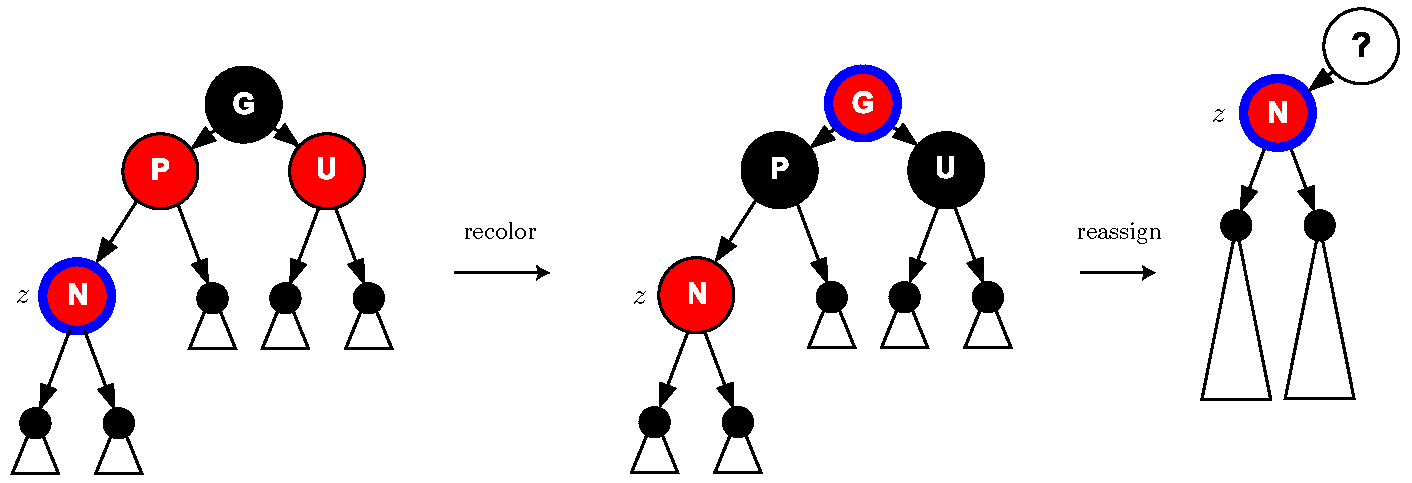
\includegraphics[width=0.9\linewidth]{rbtree_case1.pdf}
    \caption{<caption>}
    \label{fig:rbtree_case1}
\end{figure}

\subsubsection{Case 2}

\begin{figure}[htbp]
    \centering
    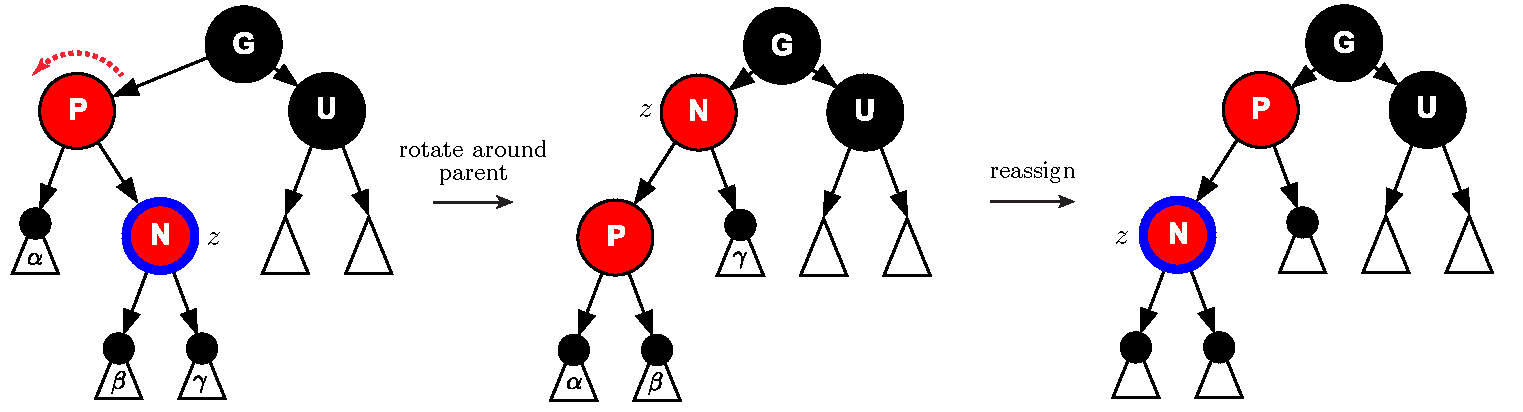
\includegraphics[width=0.9\linewidth]{rbtree_case2.pdf}
    \caption{<caption>}
    \label{fig:rbtree_case2}
\end{figure}

\subsubsection{Case 3}

\begin{figure}[htbp]
    \centering
    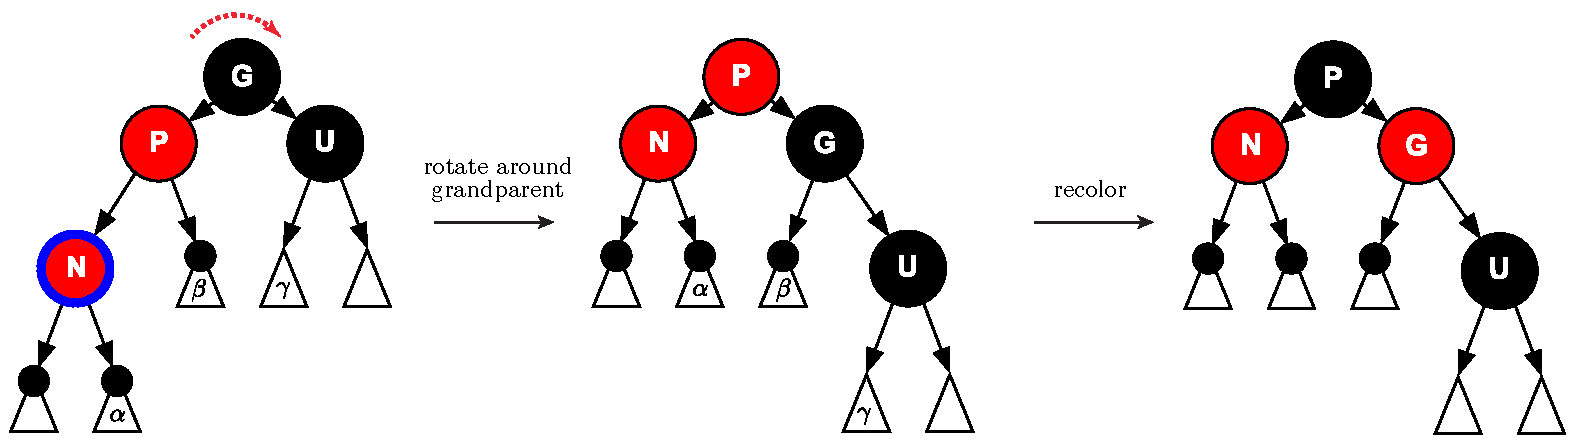
\includegraphics[width=0.9\linewidth]{rbtree_case3.pdf}
    \caption{<caption>}
    \label{fig:rbtree_case3}
\end{figure}